% Options for packages loaded elsewhere
\PassOptionsToPackage{unicode}{hyperref}
\PassOptionsToPackage{hyphens}{url}
%
\documentclass[
]{article}
\usepackage{amsmath,amssymb}
\usepackage{lmodern}
\usepackage{ifxetex,ifluatex}
\ifnum 0\ifxetex 1\fi\ifluatex 1\fi=0 % if pdftex
  \usepackage[T1]{fontenc}
  \usepackage[utf8]{inputenc}
  \usepackage{textcomp} % provide euro and other symbols
\else % if luatex or xetex
  \usepackage{unicode-math}
  \defaultfontfeatures{Scale=MatchLowercase}
  \defaultfontfeatures[\rmfamily]{Ligatures=TeX,Scale=1}
\fi
% Use upquote if available, for straight quotes in verbatim environments
\IfFileExists{upquote.sty}{\usepackage{upquote}}{}
\IfFileExists{microtype.sty}{% use microtype if available
  \usepackage[]{microtype}
  \UseMicrotypeSet[protrusion]{basicmath} % disable protrusion for tt fonts
}{}
\makeatletter
\@ifundefined{KOMAClassName}{% if non-KOMA class
  \IfFileExists{parskip.sty}{%
    \usepackage{parskip}
  }{% else
    \setlength{\parindent}{0pt}
    \setlength{\parskip}{6pt plus 2pt minus 1pt}}
}{% if KOMA class
  \KOMAoptions{parskip=half}}
\makeatother
\usepackage{xcolor}
\IfFileExists{xurl.sty}{\usepackage{xurl}}{} % add URL line breaks if available
\IfFileExists{bookmark.sty}{\usepackage{bookmark}}{\usepackage{hyperref}}
\hypersetup{
  pdftitle={Interacciones de especies: competencia!},
  pdfauthor={BIOL4558},
  hidelinks,
  pdfcreator={LaTeX via pandoc}}
\urlstyle{same} % disable monospaced font for URLs
\usepackage[margin=1in]{geometry}
\usepackage{color}
\usepackage{fancyvrb}
\newcommand{\VerbBar}{|}
\newcommand{\VERB}{\Verb[commandchars=\\\{\}]}
\DefineVerbatimEnvironment{Highlighting}{Verbatim}{commandchars=\\\{\}}
% Add ',fontsize=\small' for more characters per line
\usepackage{framed}
\definecolor{shadecolor}{RGB}{248,248,248}
\newenvironment{Shaded}{\begin{snugshade}}{\end{snugshade}}
\newcommand{\AlertTok}[1]{\textcolor[rgb]{0.94,0.16,0.16}{#1}}
\newcommand{\AnnotationTok}[1]{\textcolor[rgb]{0.56,0.35,0.01}{\textbf{\textit{#1}}}}
\newcommand{\AttributeTok}[1]{\textcolor[rgb]{0.77,0.63,0.00}{#1}}
\newcommand{\BaseNTok}[1]{\textcolor[rgb]{0.00,0.00,0.81}{#1}}
\newcommand{\BuiltInTok}[1]{#1}
\newcommand{\CharTok}[1]{\textcolor[rgb]{0.31,0.60,0.02}{#1}}
\newcommand{\CommentTok}[1]{\textcolor[rgb]{0.56,0.35,0.01}{\textit{#1}}}
\newcommand{\CommentVarTok}[1]{\textcolor[rgb]{0.56,0.35,0.01}{\textbf{\textit{#1}}}}
\newcommand{\ConstantTok}[1]{\textcolor[rgb]{0.00,0.00,0.00}{#1}}
\newcommand{\ControlFlowTok}[1]{\textcolor[rgb]{0.13,0.29,0.53}{\textbf{#1}}}
\newcommand{\DataTypeTok}[1]{\textcolor[rgb]{0.13,0.29,0.53}{#1}}
\newcommand{\DecValTok}[1]{\textcolor[rgb]{0.00,0.00,0.81}{#1}}
\newcommand{\DocumentationTok}[1]{\textcolor[rgb]{0.56,0.35,0.01}{\textbf{\textit{#1}}}}
\newcommand{\ErrorTok}[1]{\textcolor[rgb]{0.64,0.00,0.00}{\textbf{#1}}}
\newcommand{\ExtensionTok}[1]{#1}
\newcommand{\FloatTok}[1]{\textcolor[rgb]{0.00,0.00,0.81}{#1}}
\newcommand{\FunctionTok}[1]{\textcolor[rgb]{0.00,0.00,0.00}{#1}}
\newcommand{\ImportTok}[1]{#1}
\newcommand{\InformationTok}[1]{\textcolor[rgb]{0.56,0.35,0.01}{\textbf{\textit{#1}}}}
\newcommand{\KeywordTok}[1]{\textcolor[rgb]{0.13,0.29,0.53}{\textbf{#1}}}
\newcommand{\NormalTok}[1]{#1}
\newcommand{\OperatorTok}[1]{\textcolor[rgb]{0.81,0.36,0.00}{\textbf{#1}}}
\newcommand{\OtherTok}[1]{\textcolor[rgb]{0.56,0.35,0.01}{#1}}
\newcommand{\PreprocessorTok}[1]{\textcolor[rgb]{0.56,0.35,0.01}{\textit{#1}}}
\newcommand{\RegionMarkerTok}[1]{#1}
\newcommand{\SpecialCharTok}[1]{\textcolor[rgb]{0.00,0.00,0.00}{#1}}
\newcommand{\SpecialStringTok}[1]{\textcolor[rgb]{0.31,0.60,0.02}{#1}}
\newcommand{\StringTok}[1]{\textcolor[rgb]{0.31,0.60,0.02}{#1}}
\newcommand{\VariableTok}[1]{\textcolor[rgb]{0.00,0.00,0.00}{#1}}
\newcommand{\VerbatimStringTok}[1]{\textcolor[rgb]{0.31,0.60,0.02}{#1}}
\newcommand{\WarningTok}[1]{\textcolor[rgb]{0.56,0.35,0.01}{\textbf{\textit{#1}}}}
\usepackage{graphicx}
\makeatletter
\def\maxwidth{\ifdim\Gin@nat@width>\linewidth\linewidth\else\Gin@nat@width\fi}
\def\maxheight{\ifdim\Gin@nat@height>\textheight\textheight\else\Gin@nat@height\fi}
\makeatother
% Scale images if necessary, so that they will not overflow the page
% margins by default, and it is still possible to overwrite the defaults
% using explicit options in \includegraphics[width, height, ...]{}
\setkeys{Gin}{width=\maxwidth,height=\maxheight,keepaspectratio}
% Set default figure placement to htbp
\makeatletter
\def\fps@figure{htbp}
\makeatother
\setlength{\emergencystretch}{3em} % prevent overfull lines
\providecommand{\tightlist}{%
  \setlength{\itemsep}{0pt}\setlength{\parskip}{0pt}}
\setcounter{secnumdepth}{-\maxdimen} % remove section numbering
\ifluatex
  \usepackage{selnolig}  % disable illegal ligatures
\fi

\title{Interacciones de especies: competencia!}
\author{BIOL4558}
\date{Agosto 2021}

\begin{document}
\maketitle

{
\setcounter{tocdepth}{2}
\tableofcontents
}
\hypertarget{interacciones-de-especies}{%
\subsection{Interacciones de especies}\label{interacciones-de-especies}}

El PVA, como recordará, tiende a estar muy centrado en una sola especie.

PERO la ecología de la población no tiene que estar centrada en una sola
especie. Hay muchos casos en los que haríamos bien en pensar
específicamente en las interacciones de las especies.

Desde el punto de vista del modelado, aquí es donde las cosas se ponen
realmente interesantes: con las interacciones de las especies,
¡comenzamos a ver algunas propiedades emergentes realmente
impredecibles!

Las interacciones de las especies se pueden clasificar según el efecto
de la interacción en cada especie: (+, +), (+, -), (+, 0), (-, -), (-,
0), (0,0 )

\textbf{P }: ¿Puede nombrar cada una de las clases de interacción
anteriores? {[}Edmodo{]}

\hypertarget{competencia}{%
\subsection{Competencia}\label{competencia}}

\hypertarget{quuxe9-es-la-competencia}{%
\subsubsection{¿Qué es la competencia?}\label{quuxe9-es-la-competencia}}

La competencia se define como un tipo de interacción entre especies
mediante la cual \emph{las tasas vitales de población de cada especie se
ven influenciadas negativamente por la presencia de la otra }.

¡No hay mucha diferencia esencial entre la competencia dentro de las
especies (uno de los mecanismos principales para la regulación de la
población dependiente de la densidad) y la competencia entre especies
por los recursos!

\hypertarget{explotaciuxf3n}{%
\paragraph{Explotación}\label{explotaciuxf3n}}

Este es el tipo de competencia en la que probablemente pensamos primero:
todos los individuos compiten por los recursos y todos tienen
habilidades competitivas similares. Es gratis para todos: ¡todos reciben
una porción de un pastel limitado!

La competencia por los recursos dentro de las especies es a menudo el
mecanismo detrás de los procesos dependientes de la densidad que ya
hemos discutido en esta clase. Dentro de una sola especie, esto a menudo
se denomina "* competencia de revueltas *".

\hypertarget{interferencia}{%
\paragraph{Interferencia}\label{interferencia}}

A veces, el efecto negativo de un actor (individuo de la misma u otra
especie) sobre otro actor se debe a la exclusión conductual directa.
Este es el caso de las aves que mantienen territorios y mantienen a
otras aves fuera del territorio.

Algunas plantas participan en una competencia de interferencia en un
proceso llamado ``alelopatía''.

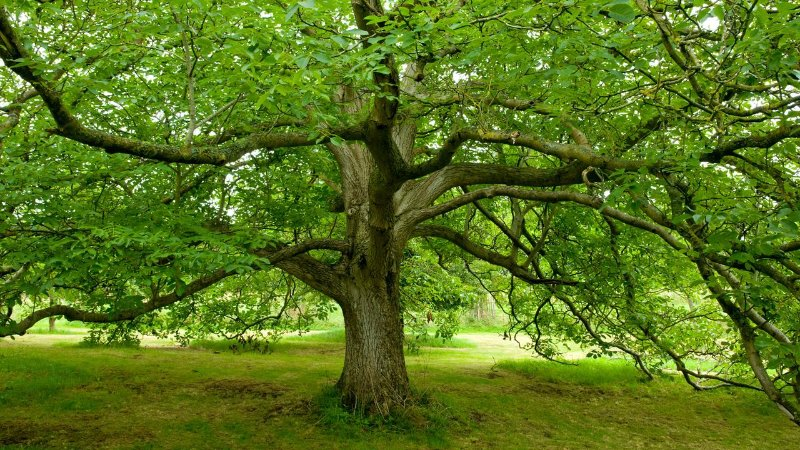
\includegraphics{figuures/allelopathy.jpg}

\hypertarget{competencia-de-modelado-extendiendo-las-ecuaciones-de-crecimiento-loguxedstico-a-muxe1s-de-una-especie}{%
\subsubsection{Competencia de modelado: ¡extendiendo las ecuaciones de
crecimiento logístico a más de una
especie!}\label{competencia-de-modelado-extendiendo-las-ecuaciones-de-crecimiento-loguxedstico-a-muxe1s-de-una-especie}}

Si * competencia entre especies * y * competencia entre especies * son
esencialmente lo mismo, ¡quizás podamos modelar estos procesos de la
misma manera!

\begin{enumerate}
\def\labelenumi{\arabic{enumi}.}
\tightlist
\item
  ¡Recuerde la ecuación de crecimiento logístico!
\end{enumerate}

\(\Delta N = r\cdot N_t \cdot (1-\frac{N}{K})\)

\begin{enumerate}
\def\labelenumi{\arabic{enumi}.}
\setcounter{enumi}{1}
\tightlist
\item
  Ahora considere el caso en el que tenemos dos especies cuya dinámica
  se puede describir mediante ecuaciones de crecimiento logístico:
\end{enumerate}

Especie 1: \(\Delta N1 = r\cdot N1_t \cdot (1-\frac{N1}{K1})\)

Especie 2: \(\Delta N2 = r\cdot N2_t \cdot (1-\frac{N2}{K2})\)

\begin{enumerate}
\def\labelenumi{\arabic{enumi}.}
\setcounter{enumi}{2}
\tightlist
\item
  ¡Ahora imagina que el crecimiento de la población de cada especie se
  deprime aún más por la presencia de la otra! Podemos imaginar un
  escenario en el que (por ejemplo,) la presencia de una especie ayude a
  * llenar * la capacidad de carga de las otras especies, ¡y viceversa!
\end{enumerate}

Especie 1: \(\Delta N1 = r\cdot N1_t \cdot (1-\frac{N1+\alpha N2}{K1})\)

Especie 2: \(\Delta N2 = r\cdot N2_t \cdot (1-\frac{N2+\beta N1}{K2})\)

Las constante \(\alpha\) y \(\beta\) son medidas del efecto de una
especie sobre el crecimiento de las otras especies.

\textbf{P }: ¿qué significa si \$ ~alpha \$ es igual a 1?

\textbf{P }: ¿qué significa si \$ ~alpha \$ es igual a 5?

\textbf{P }: ¿qué significa si \$ ~alpha \$ es igual a \$ ~frac \{1\}
\{5\} \$?

\textbf{P }: ¿qué significa si \$ ~alpha \$ es igual a cero?

\hypertarget{exploremos-este-modelo-juntos-en-insightmaker}{%
\subsubsection{Exploremos este modelo juntos en
InsightMaker!}\label{exploremos-este-modelo-juntos-en-insightmaker}}

\textbf{Paso 1 }: clone un modelo básico de dos especies (que no
interactúe) {[}aquí{]}
(\url{https://insightmaker.com/insight/77729/Base-2-species-model}).
Pruebe algunos ajustes de parámetros diferentes para asegurarse de que
el modelo está haciendo lo que espera.

\textbf{Paso 2 }: Ahora agregue los términos ``alfa'' y ``beta'' para
representar el grado en que la especie 1 compite con la especie 2, y
viceversa. * ¿A qué deberían enlazar ``alfa'' y ``beta''? *

\textbf{Paso 3 }: Cambie los valores de los parámetros y vea cómo se
comporta el modelo.

¡Este modelo se conoce como * competición Lotka-Volterra *! El modelo
lleva el nombre de los matemáticos Alfred Lotka y Vito Volterra.

\begin{quote}
\begin{quote}
\textbf{Step 1}: clone a basic (non-interacting) two-species model
\href{https://insightmaker.com/insight/77729/Base-2-species-model}{here}.
Try some different parameter settings, to make sure the model is doing
what you expect!
\end{quote}
\end{quote}

\begin{quote}
\begin{quote}
\textbf{Step 2}: Now add the ``alpha'' and ``beta'' terms to represent
the degree to which species 1 competes with species 2, and vice versa.
\emph{What should ``alpha'' and ``beta'' link to??}
\end{quote}
\end{quote}

\begin{quote}
\begin{quote}
\textbf{Step 3}: Change the parameter values around and see how the
model behaves.
\end{quote}
\end{quote}

This model is known as \emph{Lotka-Volterra competition}! The model is
named after mathematicians Alfred Lotka and Vito Volterra

\begin{center}\rule{0.5\linewidth}{0.5pt}\end{center}

\textbf{P}: Qué sucede si una especie es un competidor superior? ¿Qué
significa ser un competidor superior? ¿Puede una especie extinguirse?

\textbf{P }: ¿Qué condiciones son necesarias para la convivencia en este
modelo? {[}sombrero de copa{]}

\textbf{P }: imagina que la especie 1 es una especie exótica, un posible
invasor de un ecosistema dominado por la especie 2 (que está en
capacidad de carga). ¿Bajo qué condiciones la especie 1 tiene éxito en
la invasión? ¿En qué condiciones el invasor provoca la extinción de las
especies nativas?

\textbf{P }: ¿puede identificar alguna condición de equilibrio (estable
o inestable)?

\hypertarget{la-fase-plana}{%
\subsection{La fase plana!}\label{la-fase-plana}}

En el estudio de sistemas dinámicos (como el modelo de competición
Lotka-Volterra) puede resultar muy útil visualizar el sistema en el
\textbf{la fase plana}.

Para hacer esto, visualizamos la abundancia de cada especie que
interactúa como una coordenada en un plano cartesiano, con una especie
como eje y y la otra especie como eje x. Esta superficie 2-D se llama
plano de fase.

Luego, para cada paso de tiempo en el modelo, graficamos dónde estamos
en el plano de fase (grafica las abundancias de la especie 1 y la
especie 2 como un punto en la superficie cartesiana bidimensional).

Por ejemplo:

Construyamos el modelo básico de competencia Lotka-Volterra en R.

Si desea seguir, puede descargar el guión \href{LECTURE16.R}{aquí}

\begin{Shaded}
\begin{Highlighting}[]
\DocumentationTok{\#\#\#\#\# EJEMPLO DE COMPETICIÓN DE LOTKA VOLTERRA}

\DocumentationTok{\#\# Params}

\NormalTok{Alpha }\OtherTok{\textless{}{-}} \FloatTok{1.1}
\NormalTok{Beta }\OtherTok{\textless{}{-}} \FloatTok{0.5}
\NormalTok{InitN1 }\OtherTok{\textless{}{-}} \DecValTok{100}
\NormalTok{InitN2 }\OtherTok{\textless{}{-}} \DecValTok{300}
\NormalTok{K1 }\OtherTok{\textless{}{-}} \DecValTok{1000}
\NormalTok{K2 }\OtherTok{\textless{}{-}} \DecValTok{450}
\NormalTok{Rmax1 }\OtherTok{\textless{}{-}} \FloatTok{0.05}
\NormalTok{Rmax2 }\OtherTok{\textless{}{-}} \FloatTok{0.3}
\NormalTok{Nyears }\OtherTok{\textless{}{-}} \DecValTok{1000}

\NormalTok{System }\OtherTok{\textless{}{-}} \FunctionTok{data.frame}\NormalTok{(}\AttributeTok{n1 =} \FunctionTok{rep}\NormalTok{(InitN1,(Nyears}\SpecialCharTok{+}\DecValTok{1}\NormalTok{)),}\AttributeTok{n2 =}\NormalTok{ InitN2)}

\NormalTok{doYear }\OtherTok{\textless{}{-}} \ControlFlowTok{function}\NormalTok{(prevyear)\{}
\NormalTok{  n1 }\OtherTok{\textless{}{-}}\NormalTok{ prevyear[}\DecValTok{1}\NormalTok{] }\SpecialCharTok{+}\NormalTok{ prevyear[}\DecValTok{1}\NormalTok{] }\SpecialCharTok{*}\NormalTok{ Rmax1 }\SpecialCharTok{*}\NormalTok{ (}\DecValTok{1}\SpecialCharTok{{-}}\NormalTok{((prevyear[}\DecValTok{1}\NormalTok{]}\SpecialCharTok{+}\NormalTok{Alpha}\SpecialCharTok{*}\NormalTok{prevyear[}\DecValTok{2}\NormalTok{])}\SpecialCharTok{/}\NormalTok{(K1)))}
\NormalTok{  n2 }\OtherTok{\textless{}{-}}\NormalTok{ prevyear[}\DecValTok{2}\NormalTok{] }\SpecialCharTok{+}\NormalTok{ prevyear[}\DecValTok{2}\NormalTok{] }\SpecialCharTok{*}\NormalTok{ Rmax2 }\SpecialCharTok{*}\NormalTok{ (}\DecValTok{1}\SpecialCharTok{{-}}\NormalTok{((prevyear[}\DecValTok{2}\NormalTok{]}\SpecialCharTok{+}\NormalTok{Beta}\SpecialCharTok{*}\NormalTok{prevyear[}\DecValTok{1}\NormalTok{])}\SpecialCharTok{/}\NormalTok{(K2)))}
  \FunctionTok{return}\NormalTok{(}\FunctionTok{c}\NormalTok{(n1,n2))}
\NormalTok{\}}

\DocumentationTok{\#\# Do simulation}
\ControlFlowTok{for}\NormalTok{(i }\ControlFlowTok{in} \DecValTok{1}\SpecialCharTok{:}\NormalTok{(Nyears}\SpecialCharTok{+}\DecValTok{1}\NormalTok{))\{}
\NormalTok{  System[}\DecValTok{1}\SpecialCharTok{+}\NormalTok{i,] }\OtherTok{\textless{}{-}} \FunctionTok{doYear}\NormalTok{(System[i,])}
\NormalTok{\}}
\end{Highlighting}
\end{Shaded}

Ahora visualicemos el año cero en \emph{phase space}:

\begin{Shaded}
\begin{Highlighting}[]
\DocumentationTok{\#\#\#\#}
\CommentTok{\# visualizar las abundancias iniciales en el plano de fase}

\FunctionTok{plot}\NormalTok{(}\DecValTok{1}\NormalTok{,}\DecValTok{1}\NormalTok{,}\AttributeTok{pch=}\StringTok{""}\NormalTok{,}\AttributeTok{ylim=}\FunctionTok{c}\NormalTok{(}\DecValTok{0}\NormalTok{,K2}\SpecialCharTok{*}\FloatTok{1.5}\NormalTok{),}\AttributeTok{xlim=}\FunctionTok{c}\NormalTok{(}\DecValTok{0}\NormalTok{,K1}\SpecialCharTok{*}\FloatTok{1.5}\NormalTok{),}\AttributeTok{xlab=}\StringTok{"species 1"}\NormalTok{,}\AttributeTok{ylab=}\StringTok{"species 2"}\NormalTok{)}
\FunctionTok{points}\NormalTok{(System[}\DecValTok{1}\NormalTok{,],}\AttributeTok{col=}\StringTok{"green"}\NormalTok{,}\AttributeTok{pch=}\DecValTok{20}\NormalTok{,}\AttributeTok{cex=}\DecValTok{2}\NormalTok{)}
\end{Highlighting}
\end{Shaded}

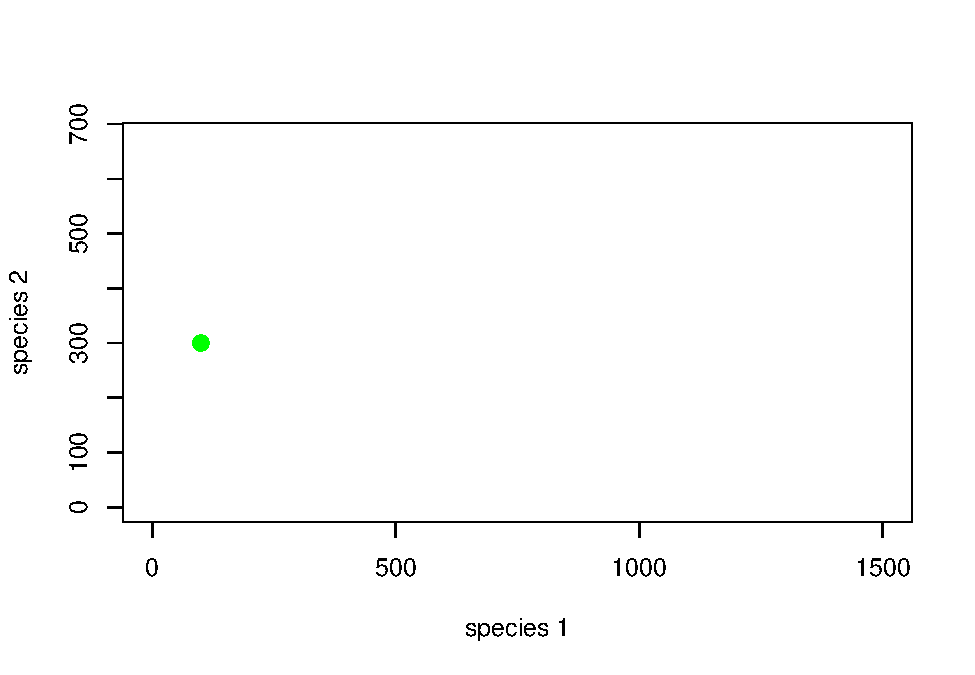
\includegraphics{LECTURE16_files/figure-latex/unnamed-chunk-3-1.pdf}

¿Qué tal los primeros 5 años \ldots{}

\begin{Shaded}
\begin{Highlighting}[]
\CommentTok{\# and the first 5 years...}
\FunctionTok{plot}\NormalTok{(}\DecValTok{1}\NormalTok{,}\DecValTok{1}\NormalTok{,}\AttributeTok{pch=}\StringTok{""}\NormalTok{,}\AttributeTok{ylim=}\FunctionTok{c}\NormalTok{(}\DecValTok{0}\NormalTok{,K2}\SpecialCharTok{*}\FloatTok{1.5}\NormalTok{),}\AttributeTok{xlim=}\FunctionTok{c}\NormalTok{(}\DecValTok{0}\NormalTok{,K1}\SpecialCharTok{*}\FloatTok{1.5}\NormalTok{),}\AttributeTok{xlab=}\StringTok{"species 1"}\NormalTok{,}\AttributeTok{ylab=}\StringTok{"species 2"}\NormalTok{)}
\FunctionTok{points}\NormalTok{(System[}\DecValTok{1}\SpecialCharTok{:}\DecValTok{6}\NormalTok{,],}\AttributeTok{col=}\StringTok{"green"}\NormalTok{,}\AttributeTok{pch=}\DecValTok{20}\NormalTok{,}\AttributeTok{cex=}\DecValTok{2}\NormalTok{)}
\end{Highlighting}
\end{Shaded}

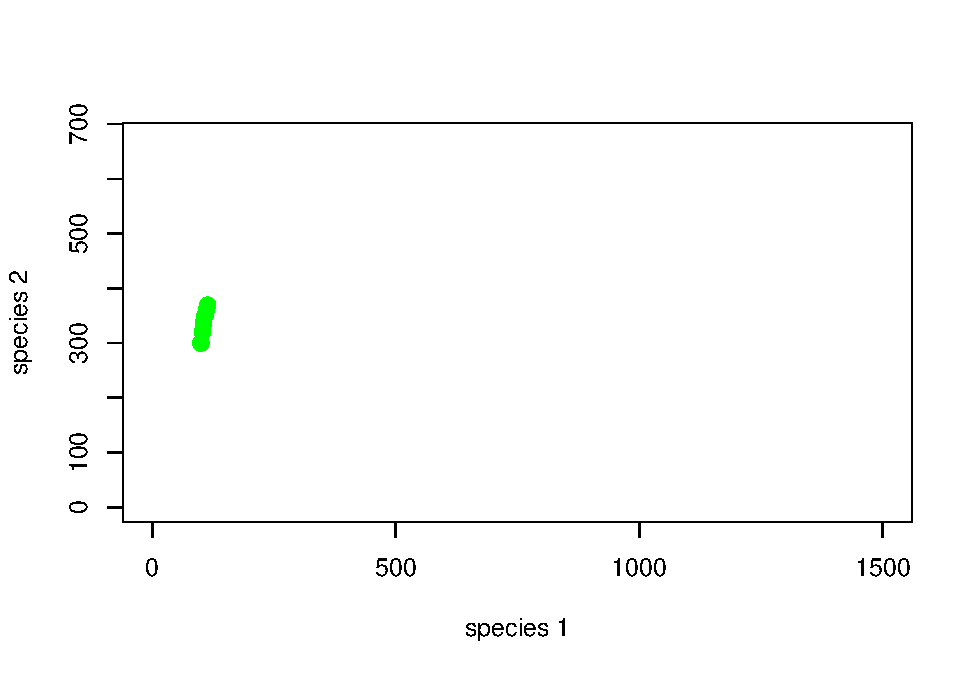
\includegraphics{LECTURE16_files/figure-latex/unnamed-chunk-4-1.pdf}

Tenga en cuenta que cada punto en el plano de fase tiene una ubicación y
una * dirección * (piense en el plano de fase como un campo magnético)
en cada punto del plano de fase, el sistema es atraído o repelido de ir
en ciertas direcciones.

¿Y toda la simulación?

\begin{Shaded}
\begin{Highlighting}[]
\CommentTok{\# and many years!}
\FunctionTok{plot}\NormalTok{(}\DecValTok{1}\NormalTok{,}\DecValTok{1}\NormalTok{,}\AttributeTok{pch=}\StringTok{""}\NormalTok{,}\AttributeTok{ylim=}\FunctionTok{c}\NormalTok{(}\DecValTok{0}\NormalTok{,K2}\SpecialCharTok{*}\FloatTok{1.5}\NormalTok{),}\AttributeTok{xlim=}\FunctionTok{c}\NormalTok{(}\DecValTok{0}\NormalTok{,K1}\SpecialCharTok{*}\FloatTok{1.5}\NormalTok{),}\AttributeTok{xlab=}\StringTok{"species 1"}\NormalTok{,}\AttributeTok{ylab=}\StringTok{"species 2"}\NormalTok{)}
\FunctionTok{points}\NormalTok{(System,}\AttributeTok{col=}\StringTok{"green"}\NormalTok{,}\AttributeTok{pch=}\DecValTok{20}\NormalTok{,}\AttributeTok{cex=}\DecValTok{2}\NormalTok{)}
\end{Highlighting}
\end{Shaded}

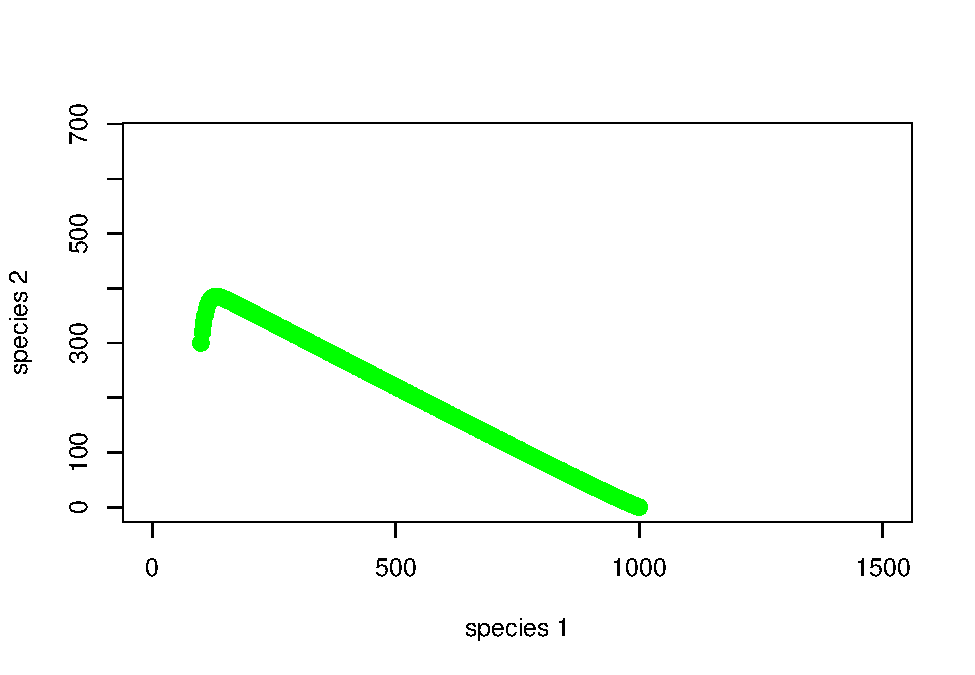
\includegraphics{LECTURE16_files/figure-latex/unnamed-chunk-5-1.pdf}

Bien, entonces la especie 1 está superando a la especie 2. ¡A medida que
aumenta la abundancia de la especie 1, la abundancia de la especie 2
disminuye y terminamos con solo la especie 1!

Aquí hay otro ejemplo \ldots{}

\begin{Shaded}
\begin{Highlighting}[]
\DocumentationTok{\#\#\#\#\# EJEMPLO DE COMPETICIÓN DE LOTKA VOLTERRA \# 2}

\DocumentationTok{\#\# Parametros}

\NormalTok{Alpha }\OtherTok{\textless{}{-}} \FloatTok{0.3}
\NormalTok{Beta }\OtherTok{\textless{}{-}} \FloatTok{0.2}
\NormalTok{InitN1 }\OtherTok{\textless{}{-}} \DecValTok{100}
\NormalTok{InitN2 }\OtherTok{\textless{}{-}} \DecValTok{300}
\NormalTok{K1 }\OtherTok{\textless{}{-}} \DecValTok{1000}
\NormalTok{K2 }\OtherTok{\textless{}{-}} \DecValTok{450}
\NormalTok{Rmax1 }\OtherTok{\textless{}{-}} \FloatTok{0.05}
\NormalTok{Rmax2 }\OtherTok{\textless{}{-}} \FloatTok{0.3}
\NormalTok{Nyears }\OtherTok{\textless{}{-}} \DecValTok{1000}

\NormalTok{System }\OtherTok{\textless{}{-}} \FunctionTok{data.frame}\NormalTok{(}\AttributeTok{n1 =} \FunctionTok{rep}\NormalTok{(InitN1,(Nyears}\SpecialCharTok{+}\DecValTok{1}\NormalTok{)),}\AttributeTok{n2 =}\NormalTok{ InitN2)}

\NormalTok{doYear }\OtherTok{\textless{}{-}} \ControlFlowTok{function}\NormalTok{(prevyear)\{}
\NormalTok{  n1 }\OtherTok{\textless{}{-}}\NormalTok{ prevyear[}\DecValTok{1}\NormalTok{] }\SpecialCharTok{+}\NormalTok{ prevyear[}\DecValTok{1}\NormalTok{] }\SpecialCharTok{*}\NormalTok{ Rmax1 }\SpecialCharTok{*}\NormalTok{ (}\DecValTok{1}\SpecialCharTok{{-}}\NormalTok{((prevyear[}\DecValTok{1}\NormalTok{]}\SpecialCharTok{+}\NormalTok{Alpha}\SpecialCharTok{*}\NormalTok{prevyear[}\DecValTok{2}\NormalTok{])}\SpecialCharTok{/}\NormalTok{(K1)))}
\NormalTok{  n2 }\OtherTok{\textless{}{-}}\NormalTok{ prevyear[}\DecValTok{2}\NormalTok{] }\SpecialCharTok{+}\NormalTok{ prevyear[}\DecValTok{2}\NormalTok{] }\SpecialCharTok{*}\NormalTok{ Rmax2 }\SpecialCharTok{*}\NormalTok{ (}\DecValTok{1}\SpecialCharTok{{-}}\NormalTok{((prevyear[}\DecValTok{2}\NormalTok{]}\SpecialCharTok{+}\NormalTok{Beta}\SpecialCharTok{*}\NormalTok{prevyear[}\DecValTok{1}\NormalTok{])}\SpecialCharTok{/}\NormalTok{(K2)))}
  \FunctionTok{return}\NormalTok{(}\FunctionTok{c}\NormalTok{(n1,n2))}
\NormalTok{\}}

\DocumentationTok{\#\# Do simulation}
\ControlFlowTok{for}\NormalTok{(i }\ControlFlowTok{in} \DecValTok{1}\SpecialCharTok{:}\NormalTok{(Nyears}\SpecialCharTok{+}\DecValTok{1}\NormalTok{))\{}
\NormalTok{  System[}\DecValTok{1}\SpecialCharTok{+}\NormalTok{i,] }\OtherTok{\textless{}{-}} \FunctionTok{doYear}\NormalTok{(System[i,])}
\NormalTok{\}}
\end{Highlighting}
\end{Shaded}

Con estos nuevos parámetros, el espacio de fase se ve así (con jittering
para indicar la concentración de puntos:

\begin{Shaded}
\begin{Highlighting}[]
\CommentTok{\# visualizar en el plano de fase}

\FunctionTok{plot}\NormalTok{(}\DecValTok{1}\NormalTok{,}\DecValTok{1}\NormalTok{,}\AttributeTok{pch=}\StringTok{""}\NormalTok{,}\AttributeTok{ylim=}\FunctionTok{c}\NormalTok{(}\DecValTok{0}\NormalTok{,K2}\SpecialCharTok{*}\FloatTok{1.5}\NormalTok{),}\AttributeTok{xlim=}\FunctionTok{c}\NormalTok{(}\DecValTok{0}\NormalTok{,K1}\SpecialCharTok{*}\FloatTok{1.5}\NormalTok{),}\AttributeTok{xlab=}\StringTok{"species 1"}\NormalTok{,}\AttributeTok{ylab=}\StringTok{"species 2"}\NormalTok{)}
\FunctionTok{points}\NormalTok{(}\FunctionTok{jitter}\NormalTok{(System[,}\DecValTok{1}\NormalTok{],}\DecValTok{500}\NormalTok{),}\FunctionTok{jitter}\NormalTok{(System[,}\DecValTok{2}\NormalTok{],}\DecValTok{500}\NormalTok{),}\AttributeTok{col=}\StringTok{"brown"}\NormalTok{,}\AttributeTok{pch=}\DecValTok{20}\NormalTok{,}\AttributeTok{cex=}\FloatTok{0.3}\NormalTok{)}
\FunctionTok{abline}\NormalTok{(}\AttributeTok{h=}\NormalTok{K2,}\AttributeTok{v=}\NormalTok{K1,}\AttributeTok{col=}\StringTok{"gray"}\NormalTok{,}\AttributeTok{lwd=}\DecValTok{2}\NormalTok{,}\AttributeTok{lty=}\DecValTok{2}\NormalTok{)}
\end{Highlighting}
\end{Shaded}

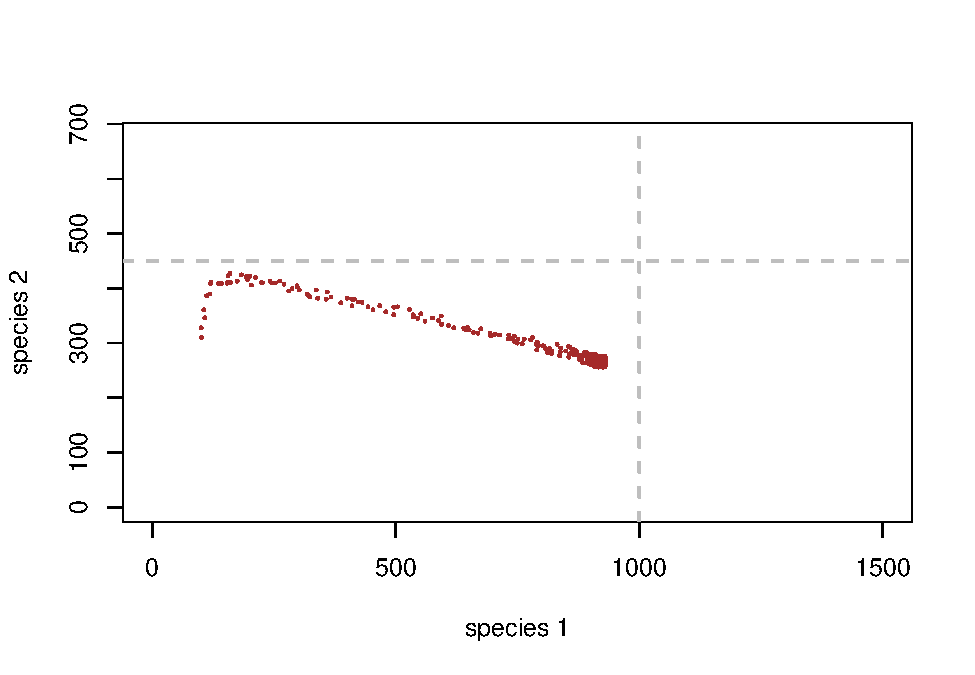
\includegraphics{LECTURE16_files/figure-latex/unnamed-chunk-7-1.pdf}

Puede ver que este sistema ha llegado a un equilibrio al final, justo
por debajo de la capacidad de carga de la especie 1.

Finalmente, consideremos múltiples puntos de partida y veamos cómo se
comporta el sistema.!

\begin{Shaded}
\begin{Highlighting}[]
\DocumentationTok{\#\#\#\#\# EJEMPLO DE COMPETICIÓN DE LOTKA VOLTERRA \# 3: múltiples puntos de partida}

\DocumentationTok{\#\# Parametros}


\NormalTok{InitN1 }\OtherTok{\textless{}{-}} \DecValTok{1200}
\NormalTok{InitN2 }\OtherTok{\textless{}{-}} \DecValTok{25}
\NormalTok{System1 }\OtherTok{\textless{}{-}} \FunctionTok{data.frame}\NormalTok{(}\AttributeTok{n1 =} \FunctionTok{rep}\NormalTok{(InitN1,(Nyears}\SpecialCharTok{+}\DecValTok{1}\NormalTok{)),}\AttributeTok{n2 =}\NormalTok{ InitN2)}
\DocumentationTok{\#\# Do simulation}
\ControlFlowTok{for}\NormalTok{(i }\ControlFlowTok{in} \DecValTok{1}\SpecialCharTok{:}\NormalTok{(Nyears}\SpecialCharTok{+}\DecValTok{1}\NormalTok{))\{}
\NormalTok{  System1[}\DecValTok{1}\SpecialCharTok{+}\NormalTok{i,] }\OtherTok{\textless{}{-}} \FunctionTok{doYear}\NormalTok{(System1[i,])}
\NormalTok{\}}

\NormalTok{InitN1 }\OtherTok{\textless{}{-}} \DecValTok{500}
\NormalTok{InitN2 }\OtherTok{\textless{}{-}} \DecValTok{100}
\NormalTok{System2 }\OtherTok{\textless{}{-}} \FunctionTok{data.frame}\NormalTok{(}\AttributeTok{n1 =} \FunctionTok{rep}\NormalTok{(InitN1,(Nyears}\SpecialCharTok{+}\DecValTok{1}\NormalTok{)),}\AttributeTok{n2 =}\NormalTok{ InitN2)}
\DocumentationTok{\#\# Do simulation}
\ControlFlowTok{for}\NormalTok{(i }\ControlFlowTok{in} \DecValTok{1}\SpecialCharTok{:}\NormalTok{(Nyears}\SpecialCharTok{+}\DecValTok{1}\NormalTok{))\{}
\NormalTok{  System2[}\DecValTok{1}\SpecialCharTok{+}\NormalTok{i,] }\OtherTok{\textless{}{-}} \FunctionTok{doYear}\NormalTok{(System2[i,])}
\NormalTok{\}}


\NormalTok{InitN1 }\OtherTok{\textless{}{-}} \DecValTok{800}
\NormalTok{InitN2 }\OtherTok{\textless{}{-}} \DecValTok{600}
\NormalTok{System3 }\OtherTok{\textless{}{-}} \FunctionTok{data.frame}\NormalTok{(}\AttributeTok{n1 =} \FunctionTok{rep}\NormalTok{(InitN1,(Nyears}\SpecialCharTok{+}\DecValTok{1}\NormalTok{)),}\AttributeTok{n2 =}\NormalTok{ InitN2)}
\DocumentationTok{\#\# Do simulation}
\ControlFlowTok{for}\NormalTok{(i }\ControlFlowTok{in} \DecValTok{1}\SpecialCharTok{:}\NormalTok{(Nyears}\SpecialCharTok{+}\DecValTok{1}\NormalTok{))\{}
\NormalTok{  System3[}\DecValTok{1}\SpecialCharTok{+}\NormalTok{i,] }\OtherTok{\textless{}{-}} \FunctionTok{doYear}\NormalTok{(System3[i,])}
\NormalTok{\}}
\end{Highlighting}
\end{Shaded}

Ahora, el espacio de fase se ve así (con jittering para indicar la
concentración de puntos:

\begin{Shaded}
\begin{Highlighting}[]
\CommentTok{\# visualizar en el plano de fase}

\FunctionTok{plot}\NormalTok{(}\DecValTok{1}\NormalTok{,}\DecValTok{1}\NormalTok{,}\AttributeTok{pch=}\StringTok{""}\NormalTok{,}\AttributeTok{ylim=}\FunctionTok{c}\NormalTok{(}\DecValTok{0}\NormalTok{,K2}\SpecialCharTok{*}\FloatTok{1.5}\NormalTok{),}\AttributeTok{xlim=}\FunctionTok{c}\NormalTok{(}\DecValTok{0}\NormalTok{,K1}\SpecialCharTok{*}\FloatTok{1.5}\NormalTok{),}\AttributeTok{xlab=}\StringTok{"species 1"}\NormalTok{,}\AttributeTok{ylab=}\StringTok{"species 2"}\NormalTok{)}
\FunctionTok{points}\NormalTok{(}\FunctionTok{jitter}\NormalTok{(System[,}\DecValTok{1}\NormalTok{],}\DecValTok{500}\NormalTok{),}\FunctionTok{jitter}\NormalTok{(System[,}\DecValTok{2}\NormalTok{],}\DecValTok{500}\NormalTok{),}\AttributeTok{col=}\StringTok{"brown"}\NormalTok{,}\AttributeTok{pch=}\DecValTok{20}\NormalTok{,}\AttributeTok{cex=}\FloatTok{0.3}\NormalTok{)}
\FunctionTok{points}\NormalTok{(}\FunctionTok{jitter}\NormalTok{(System1[,}\DecValTok{1}\NormalTok{],}\DecValTok{500}\NormalTok{),}\FunctionTok{jitter}\NormalTok{(System1[,}\DecValTok{2}\NormalTok{],}\DecValTok{500}\NormalTok{),}\AttributeTok{col=}\StringTok{"green"}\NormalTok{,}\AttributeTok{pch=}\DecValTok{20}\NormalTok{,}\AttributeTok{cex=}\FloatTok{0.3}\NormalTok{)}
\FunctionTok{points}\NormalTok{(}\FunctionTok{jitter}\NormalTok{(System2[,}\DecValTok{1}\NormalTok{],}\DecValTok{500}\NormalTok{),}\FunctionTok{jitter}\NormalTok{(System2[,}\DecValTok{2}\NormalTok{],}\DecValTok{500}\NormalTok{),}\AttributeTok{col=}\StringTok{"red"}\NormalTok{,}\AttributeTok{pch=}\DecValTok{20}\NormalTok{,}\AttributeTok{cex=}\FloatTok{0.3}\NormalTok{)}
\FunctionTok{points}\NormalTok{(}\FunctionTok{jitter}\NormalTok{(System3[,}\DecValTok{1}\NormalTok{],}\DecValTok{500}\NormalTok{),}\FunctionTok{jitter}\NormalTok{(System3[,}\DecValTok{2}\NormalTok{],}\DecValTok{500}\NormalTok{),}\AttributeTok{col=}\StringTok{"blue"}\NormalTok{,}\AttributeTok{pch=}\DecValTok{20}\NormalTok{,}\AttributeTok{cex=}\FloatTok{0.3}\NormalTok{)}

\FunctionTok{abline}\NormalTok{(}\AttributeTok{h=}\NormalTok{K2,}\AttributeTok{v=}\NormalTok{K1,}\AttributeTok{col=}\StringTok{"gray"}\NormalTok{,}\AttributeTok{lwd=}\DecValTok{2}\NormalTok{,}\AttributeTok{lty=}\DecValTok{2}\NormalTok{)}
\end{Highlighting}
\end{Shaded}

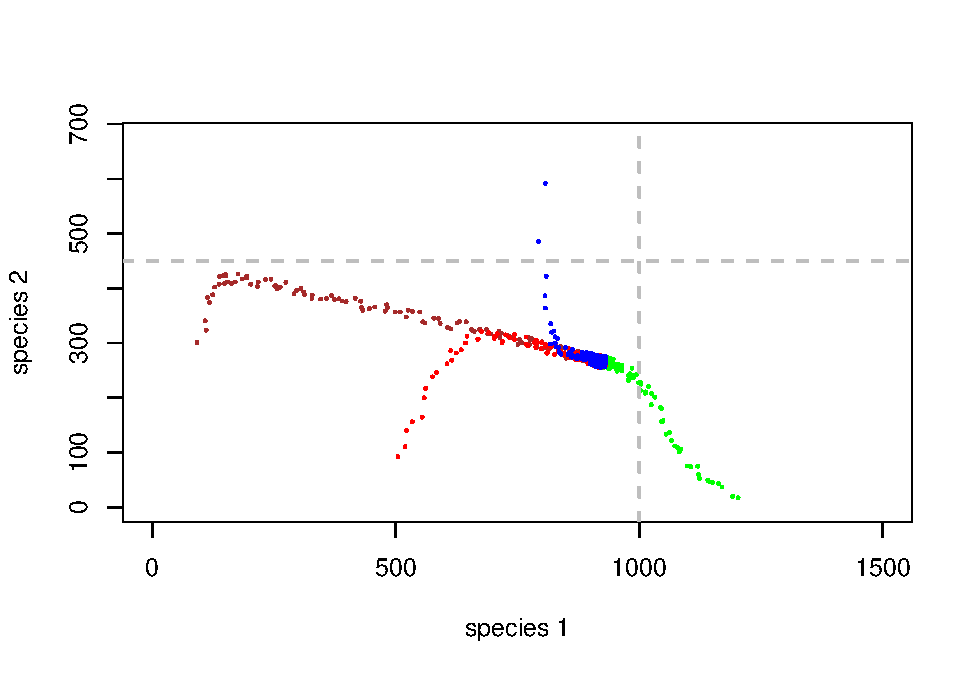
\includegraphics{LECTURE16_files/figure-latex/unnamed-chunk-9-1.pdf}

\textbf{P }: ¿Tiene este sistema de dos especies un equilibrio estable?

\hypertarget{trabajando-en-el-plano-de-fase}{%
\subsubsection{¡Trabajando en el plano de
fase!}\label{trabajando-en-el-plano-de-fase}}

Hay mucho que puede aprender sobre un sistema de dos especies que
interactúan trabajando con el plano de fase.

En primer lugar, es útil imaginar que cada punto en el espacio de fase
está asociado con una flecha, que indica hacia dónde se espera que vaya
el sistema desde ese punto en el espacio de fase (cada punto tiene una
dirección asociada).

Entonces, imagina que comenzamos con la abundancia inicial en las
figuras anteriores. ¿Dónde apunta la flecha en el espacio de fase?

La * longitud * de la flecha representa la velocidad a la que el sistema
se moverá en la dirección de la flecha (el grado de * repulsión * desde
ese punto en el espacio de fase).

Ahora imagine que dibujamos flechas a lo largo del espacio de fase, que
representan hacia dónde se espera que vaya el sistema.

Nota: este ejemplo usa código R de
\href{http://www.pauljhurtado.com/}{Paul Hurtado}

\begin{Shaded}
\begin{Highlighting}[]
\DocumentationTok{\#\#\#\#\#\#\#\#\#\#}
\CommentTok{\# ¡Visualice el plano de fase con flechas!}
\DocumentationTok{\#\#\#\#\#\#\#\#\#\#}

\DocumentationTok{\#\#\#\#\#\#\#\#\#\#\#\#\#\#\#\#\#\#\#\#\#\#\#\#\#\#\#\#\#\#\#\#\#\#\#\#\#\#\#\#\#\#\#\#\#\#\#\#\#\#\#\#\#\#\#\#\#\#\#\#\#\#\#\#\#\#\#\#\#\#\#\#\#\#\#\#\#\#\#\#\#\#\#\#\#\#\#}
\DocumentationTok{\#\# SPECIFY MODEL AND INITIALIZE}
\CommentTok{\#}
\DocumentationTok{\#\# toggle switch function for phase arrow and nullcline plotting }

\NormalTok{toggle }\OtherTok{=}\NormalTok{ compiler}\SpecialCharTok{::}\FunctionTok{cmpfun}\NormalTok{(}\ControlFlowTok{function}\NormalTok{(u,v,parms) \{}
  \FunctionTok{c}\NormalTok{( u}\SpecialCharTok{*}\NormalTok{parms[}\DecValTok{1}\NormalTok{]}\SpecialCharTok{*}\NormalTok{(}\DecValTok{1}\SpecialCharTok{{-}}\NormalTok{(u}\SpecialCharTok{+}\NormalTok{(parms[}\DecValTok{2}\NormalTok{]}\SpecialCharTok{*}\NormalTok{v))}\SpecialCharTok{/}\NormalTok{parms[}\DecValTok{3}\NormalTok{]), v}\SpecialCharTok{*}\NormalTok{parms[}\DecValTok{4}\NormalTok{]}\SpecialCharTok{*}\NormalTok{(}\DecValTok{1}\SpecialCharTok{{-}}\NormalTok{(v}\SpecialCharTok{+}\NormalTok{(parms[}\DecValTok{5}\NormalTok{]}\SpecialCharTok{*}\NormalTok{u))}\SpecialCharTok{/}\NormalTok{parms[}\DecValTok{6}\NormalTok{]) )}
\NormalTok{\})}

\NormalTok{fun}\OtherTok{=}\NormalTok{toggle }\DocumentationTok{\#\# Our generic name for the system of equations to look at! ;{-})}
\CommentTok{\#}
\DocumentationTok{\#\# toggle switch function for computing solution trajectories with deSolve::ode()}

\CommentTok{\#Toggle = as.ode.func(toggle)}
\CommentTok{\#}
\DocumentationTok{\#\# parameter values?}

\NormalTok{Rmax1 }\OtherTok{\textless{}{-}} \FloatTok{0.05}
\NormalTok{Alpha }\OtherTok{\textless{}{-}} \FloatTok{0.3}
\NormalTok{K1 }\OtherTok{\textless{}{-}} \DecValTok{1000}
\NormalTok{Rmax2 }\OtherTok{\textless{}{-}} \FloatTok{0.3}
\NormalTok{Beta }\OtherTok{\textless{}{-}} \FloatTok{0.2}
\NormalTok{K2 }\OtherTok{\textless{}{-}} \DecValTok{450}

\NormalTok{parms}\OtherTok{=}\FunctionTok{c}\NormalTok{(Rmax1,Alpha,K1,Rmax2,Beta,K2)}

\CommentTok{\# toggle(100,100,parms)}

\NormalTok{xlim }\OtherTok{=} \FunctionTok{c}\NormalTok{(}\DecValTok{5}\NormalTok{,}\DecValTok{2000}\NormalTok{)}
\NormalTok{ylim }\OtherTok{=} \FunctionTok{c}\NormalTok{(}\DecValTok{5}\NormalTok{,}\DecValTok{1000}\NormalTok{)}
\NormalTok{new }\OtherTok{\textless{}{-}} \FunctionTok{phasearrows.calc}\NormalTok{(toggle,xlim,ylim,}\AttributeTok{resol=}\DecValTok{25}\NormalTok{,}\AttributeTok{parms=}\NormalTok{parms)}

\FunctionTok{plot}\NormalTok{(}\DecValTok{1}\NormalTok{,}\DecValTok{1}\NormalTok{,}\AttributeTok{pch=}\StringTok{""}\NormalTok{,}\AttributeTok{xlim=}\NormalTok{xlim,}\AttributeTok{ylim=}\NormalTok{ylim,}\AttributeTok{xlab=}\StringTok{"N1"}\NormalTok{,}\AttributeTok{ylab=}\StringTok{"N2"}\NormalTok{)}
\FunctionTok{phasearrows.draw}\NormalTok{(new)}
\end{Highlighting}
\end{Shaded}

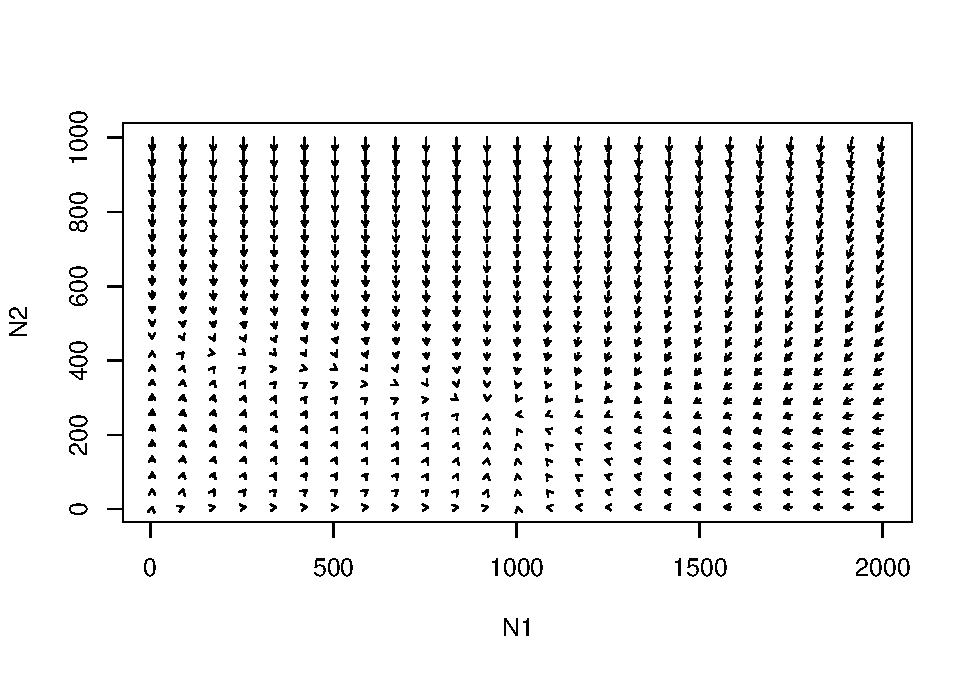
\includegraphics{LECTURE16_files/figure-latex/unnamed-chunk-11-1.pdf}

\begin{Shaded}
\begin{Highlighting}[]
\CommentTok{\#}
\DocumentationTok{\#\# }\RegionMarkerTok{END}\DocumentationTok{ MODEL SPECIFICATION AND INITIALIZATION}
\DocumentationTok{\#\#\#\#\#\#\#\#\#\#\#\#\#\#\#\#\#\#\#\#\#\#\#\#\#\#\#\#\#\#\#\#\#\#\#\#\#\#\#\#\#\#\#\#\#\#\#\#\#\#\#\#\#\#\#\#\#\#\#\#\#\#\#\#\#\#\#\#\#\#\#\#\#\#\#\#\#\#\#\#\#\#\#\#\#\#\#}
\end{Highlighting}
\end{Shaded}

Tome cualquier punto de partida arbitrario. Ahora podemos rastrear la
trayectoria que tomará el sistema en el espacio de fase.

¡¡Intentalo!!

Verá que hay algunos umbrales clave en el espacio de fase que debemos
considerar. Por ejemplo, las flechas pueden invertir la dirección.

\hypertarget{isoclinas}{%
\subsubsection{Isoclinas!}\label{isoclinas}}

Las isoclinas ayudan a delinear esas características clave en el espacio
de fase, algo así como las cimas de las montañas. ¡El lugar más allá del
cual las flechas hacia arriba se convierten en flechas hacia abajo!

He aquí un ejemplo:

\hypertarget{especie-1-isoclina}{%
\paragraph{Especie 1 isoclina \ldots{}}\label{especie-1-isoclina}}

\begin{Shaded}
\begin{Highlighting}[]
\DocumentationTok{\#\#\#\# example with phase{-}plane arrows}

\FunctionTok{plot}\NormalTok{(}\DecValTok{1}\NormalTok{,}\DecValTok{1}\NormalTok{,}\AttributeTok{pch=}\StringTok{""}\NormalTok{,}\AttributeTok{xlim=}\NormalTok{xlim,}\AttributeTok{ylim=}\NormalTok{ylim,}\AttributeTok{xlab=}\StringTok{"N1"}\NormalTok{,}\AttributeTok{ylab=}\StringTok{"N2"}\NormalTok{)}
\FunctionTok{phasearrows.draw}\NormalTok{(new)}
\FunctionTok{abline}\NormalTok{(K1}\SpecialCharTok{/}\NormalTok{Alpha,}\SpecialCharTok{{-}}\NormalTok{(K1}\SpecialCharTok{/}\NormalTok{Alpha)}\SpecialCharTok{/}\NormalTok{K1,}\AttributeTok{col=}\StringTok{"red"}\NormalTok{,}\AttributeTok{lwd=}\DecValTok{3}\NormalTok{)   }\CommentTok{\# species 1}
\FunctionTok{abline}\NormalTok{(K2,}\SpecialCharTok{{-}}\NormalTok{K2}\SpecialCharTok{/}\NormalTok{(K2}\SpecialCharTok{/}\NormalTok{Beta),}\AttributeTok{col=}\StringTok{"blue"}\NormalTok{,}\AttributeTok{lwd=}\DecValTok{3}\NormalTok{)   }\CommentTok{\# species 1}
\end{Highlighting}
\end{Shaded}

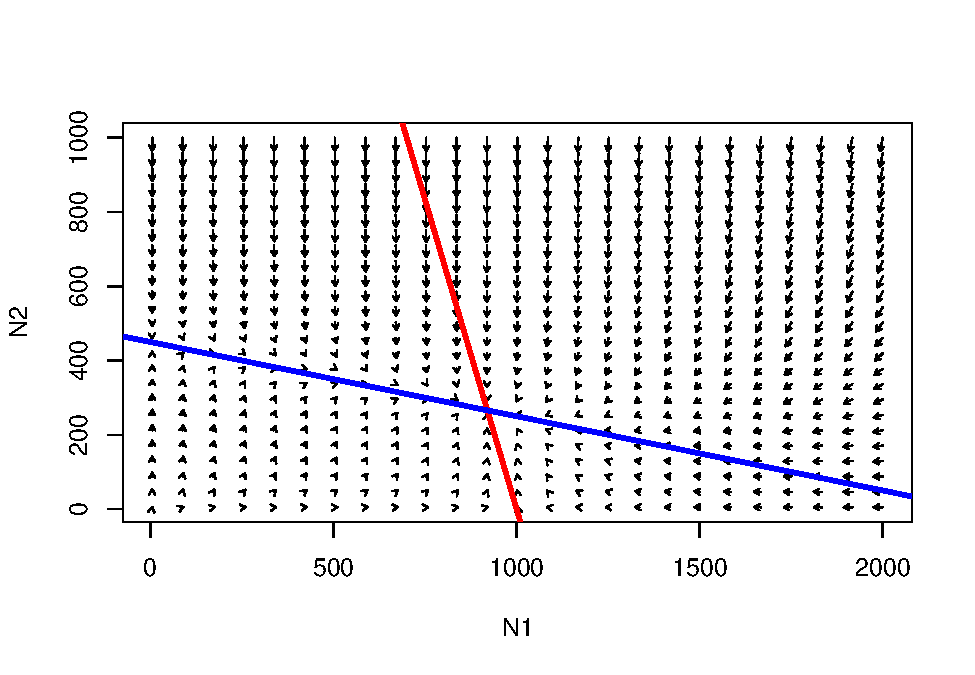
\includegraphics{LECTURE16_files/figure-latex/unnamed-chunk-12-1.pdf}

La línea roja representa las condiciones bajo las cuales la tasa de
crecimiento de la especie 1 es cero.

\textbf{P }: ¿bajo qué condiciones se ``agota'' la capacidad de carga
para la especie 1?

Por debajo de la línea roja, la especie 1 tenderá a aumentar.

Por encima de la línea roja, la especie 1 tenderá a disminuir.

¡La línea azul (isoclina) representa las condiciones bajo las cuales se
agota la capacidad de carga de la especie 2!

\textbf{P }: ¿bajo qué condiciones se ``agota'' la capacidad de carga
para la especie 2?

Por debajo de la línea azul, la especie 2 tenderá a aumentar.

Por encima de la línea azul, la especie 2 tenderá a disminuir.

\textbf{Q }: considere el punto donde se cruzan las dos isoclinas. ¿Qué
representa este punto? {[}Edmodo{]}

Consideremos el siguiente caso \ldots{}

\begin{Shaded}
\begin{Highlighting}[]
\DocumentationTok{\#\#\#\#\#\#\#\#\#\#}
\CommentTok{\# Another example}
\DocumentationTok{\#\#\#\#\#\#\#\#\#\#}

\NormalTok{Rmax1 }\OtherTok{\textless{}{-}} \FloatTok{0.2}
\NormalTok{Alpha }\OtherTok{\textless{}{-}} \FloatTok{1.1}
\NormalTok{K1 }\OtherTok{\textless{}{-}} \DecValTok{1000}
\NormalTok{Rmax2 }\OtherTok{\textless{}{-}} \FloatTok{0.2}
\NormalTok{Beta }\OtherTok{\textless{}{-}} \FloatTok{0.9}
\NormalTok{K2 }\OtherTok{\textless{}{-}} \DecValTok{500}

\NormalTok{parms}\OtherTok{=}\FunctionTok{c}\NormalTok{(Rmax1,Alpha,K1,Rmax2,Beta,K2)}

\CommentTok{\# toggle(100,100,parms)}

\NormalTok{xlim }\OtherTok{=} \FunctionTok{c}\NormalTok{(}\DecValTok{5}\NormalTok{,}\DecValTok{1500}\NormalTok{)}
\NormalTok{ylim }\OtherTok{=} \FunctionTok{c}\NormalTok{(}\DecValTok{5}\NormalTok{,}\DecValTok{1000}\NormalTok{)}
\NormalTok{new }\OtherTok{\textless{}{-}} \FunctionTok{phasearrows.calc}\NormalTok{(toggle,xlim,ylim,}\AttributeTok{resol=}\DecValTok{25}\NormalTok{,}\AttributeTok{parms=}\NormalTok{parms)}

\FunctionTok{plot}\NormalTok{(}\DecValTok{1}\NormalTok{,}\DecValTok{1}\NormalTok{,}\AttributeTok{pch=}\StringTok{""}\NormalTok{,}\AttributeTok{xlim=}\NormalTok{xlim,}\AttributeTok{ylim=}\NormalTok{ylim,}\AttributeTok{xlab=}\StringTok{"N1"}\NormalTok{,}\AttributeTok{ylab=}\StringTok{"N2"}\NormalTok{)}
\FunctionTok{phasearrows.draw}\NormalTok{(new)}
\FunctionTok{abline}\NormalTok{(K1}\SpecialCharTok{/}\NormalTok{Alpha,}\SpecialCharTok{{-}}\NormalTok{(K1}\SpecialCharTok{/}\NormalTok{Alpha)}\SpecialCharTok{/}\NormalTok{K1,}\AttributeTok{col=}\StringTok{"red"}\NormalTok{,}\AttributeTok{lwd=}\DecValTok{3}\NormalTok{)   }\CommentTok{\# species 1}
\FunctionTok{abline}\NormalTok{(K2,}\SpecialCharTok{{-}}\NormalTok{K2}\SpecialCharTok{/}\NormalTok{(K2}\SpecialCharTok{/}\NormalTok{Beta),}\AttributeTok{col=}\StringTok{"blue"}\NormalTok{,}\AttributeTok{lwd=}\DecValTok{3}\NormalTok{)   }\CommentTok{\# species 2}
\end{Highlighting}
\end{Shaded}

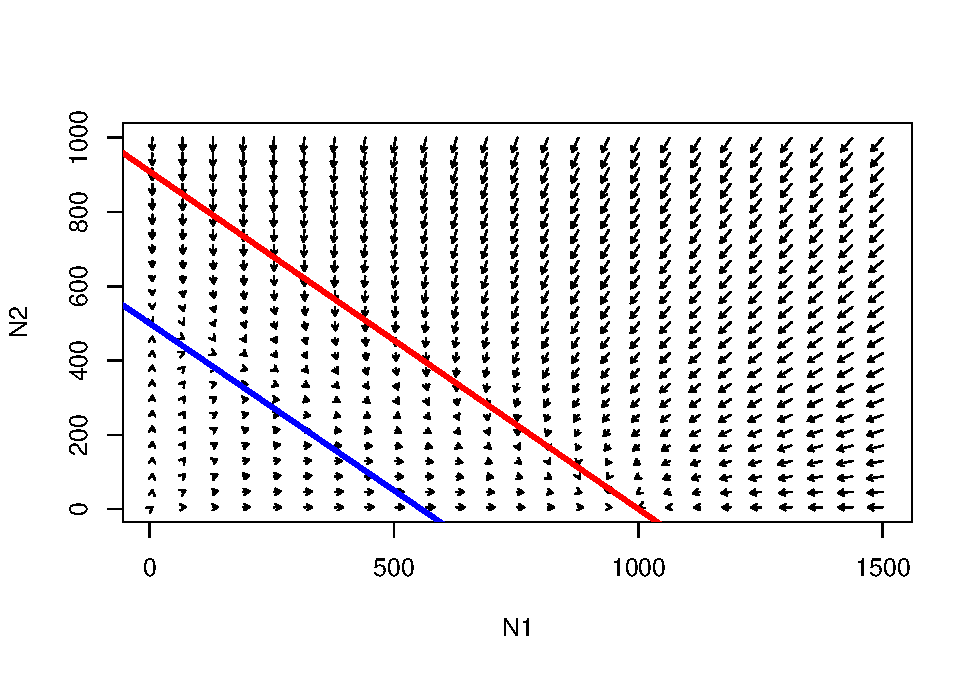
\includegraphics{LECTURE16_files/figure-latex/unnamed-chunk-13-1.pdf}

Siga las trayectorias desde cualquier punto en este espacio de fase.
¿Cuál es el resultado aquí?

\textbf{P }: ¿Existe un equilibrio en todo el sistema? {[}sombrero de
copa{]}

\textbf{P }: ¿Hay algún punto en este espacio de fase en el que el
crecimiento de la población sea negativo para la especie 1 (K1 agotado)
y positivo para la especie 2 (parte del K2 sin uso)?

\textbf{P }: ¿Qué sucede con la especie 1 cuando la capacidad de carga
se agota para la especie 2? ¿Hay espacio para la invasión de la especie
1?

\textbf{P }: ¿Qué sucede con la especie 2 cuando la capacidad de carga
se agota para la especie 1? ¿Hay espacio para la invasión de la especie
2?

¿Qué tal este ejemplo?

\begin{Shaded}
\begin{Highlighting}[]
\DocumentationTok{\#\#\#\#\#\#\#\#\#}
\CommentTok{\# And another example!}
\DocumentationTok{\#\#\#\#\#\#\#\#\#}

\NormalTok{Rmax1 }\OtherTok{\textless{}{-}} \FloatTok{0.5}
\NormalTok{Alpha }\OtherTok{\textless{}{-}} \FloatTok{1.05}
\NormalTok{K1 }\OtherTok{\textless{}{-}} \DecValTok{890}
\NormalTok{Rmax2 }\OtherTok{\textless{}{-}} \FloatTok{0.2}
\NormalTok{Beta }\OtherTok{\textless{}{-}} \FloatTok{0.5}
\NormalTok{K2 }\OtherTok{\textless{}{-}} \DecValTok{890}

\NormalTok{parms}\OtherTok{=}\FunctionTok{c}\NormalTok{(Rmax1,Alpha,K1,Rmax2,Beta,K2)}

\CommentTok{\# toggle(100,100,parms)}

\NormalTok{xlim }\OtherTok{=} \FunctionTok{c}\NormalTok{(}\DecValTok{5}\NormalTok{,}\DecValTok{1500}\NormalTok{)}
\NormalTok{ylim }\OtherTok{=} \FunctionTok{c}\NormalTok{(}\DecValTok{5}\NormalTok{,}\DecValTok{1000}\NormalTok{)}
\NormalTok{new }\OtherTok{\textless{}{-}} \FunctionTok{phasearrows.calc}\NormalTok{(toggle,xlim,ylim,}\AttributeTok{resol=}\DecValTok{25}\NormalTok{,}\AttributeTok{parms=}\NormalTok{parms)}

\FunctionTok{plot}\NormalTok{(}\DecValTok{1}\NormalTok{,}\DecValTok{1}\NormalTok{,}\AttributeTok{pch=}\StringTok{""}\NormalTok{,}\AttributeTok{xlim=}\NormalTok{xlim,}\AttributeTok{ylim=}\NormalTok{ylim,}\AttributeTok{xlab=}\StringTok{"N1"}\NormalTok{,}\AttributeTok{ylab=}\StringTok{"N2"}\NormalTok{)}
\FunctionTok{phasearrows.draw}\NormalTok{(new)}
\FunctionTok{abline}\NormalTok{(K1}\SpecialCharTok{/}\NormalTok{Alpha,}\SpecialCharTok{{-}}\NormalTok{(K1}\SpecialCharTok{/}\NormalTok{Alpha)}\SpecialCharTok{/}\NormalTok{K1,}\AttributeTok{col=}\StringTok{"red"}\NormalTok{,}\AttributeTok{lwd=}\DecValTok{3}\NormalTok{)   }\CommentTok{\# species 1}
\FunctionTok{abline}\NormalTok{(K2,}\SpecialCharTok{{-}}\NormalTok{K2}\SpecialCharTok{/}\NormalTok{(K2}\SpecialCharTok{/}\NormalTok{Beta),}\AttributeTok{col=}\StringTok{"blue"}\NormalTok{,}\AttributeTok{lwd=}\DecValTok{3}\NormalTok{)   }\CommentTok{\# species 2}
\end{Highlighting}
\end{Shaded}

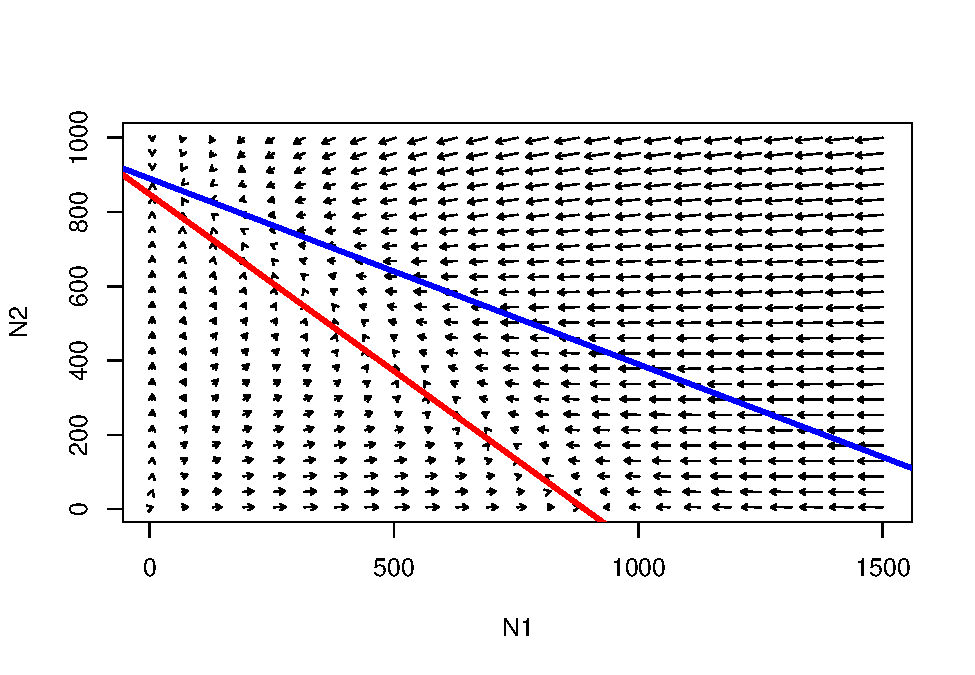
\includegraphics{LECTURE16_files/figure-latex/unnamed-chunk-14-1.pdf}

Siga las trayectorias desde cualquier punto en este espacio de fase.
¿Cuál es el resultado aquí?

** P **: ¿Existe un equilibrio en todo el sistema?

¿Qué pasa con este caso (volviendo al ejemplo anterior \ldots):

\begin{Shaded}
\begin{Highlighting}[]
\DocumentationTok{\#\#\#\#\#\#\#\#}
\CommentTok{\# And another!}
\DocumentationTok{\#\#\#\#\#\#\#\#\#}

\NormalTok{Alpha }\OtherTok{\textless{}{-}} \FloatTok{0.3}
\NormalTok{Beta }\OtherTok{\textless{}{-}} \FloatTok{0.2}
\NormalTok{K1 }\OtherTok{\textless{}{-}} \DecValTok{1000}
\NormalTok{K2 }\OtherTok{\textless{}{-}} \DecValTok{450}
\NormalTok{Rmax1 }\OtherTok{\textless{}{-}} \FloatTok{0.05}
\NormalTok{Rmax2 }\OtherTok{\textless{}{-}} \FloatTok{0.3}
\NormalTok{Nyears }\OtherTok{\textless{}{-}} \DecValTok{1000}
\NormalTok{ylim}\OtherTok{=}\FunctionTok{c}\NormalTok{(}\DecValTok{0}\NormalTok{,K2}\SpecialCharTok{*}\FloatTok{1.5}\NormalTok{)}
\NormalTok{xlim}\OtherTok{=}\FunctionTok{c}\NormalTok{(}\DecValTok{0}\NormalTok{,K1}\SpecialCharTok{*}\FloatTok{1.5}\NormalTok{)}
\FunctionTok{plot}\NormalTok{(}\DecValTok{1}\NormalTok{,}\DecValTok{1}\NormalTok{,}\AttributeTok{pch=}\StringTok{""}\NormalTok{,}\AttributeTok{ylim=}\NormalTok{ylim,}\AttributeTok{xlim=}\NormalTok{xlim,}\AttributeTok{xlab=}\StringTok{"species 1"}\NormalTok{,}\AttributeTok{ylab=}\StringTok{"species 2"}\NormalTok{)}
\FunctionTok{points}\NormalTok{(}\FunctionTok{jitter}\NormalTok{(System[,}\DecValTok{1}\NormalTok{],}\DecValTok{500}\NormalTok{),}\FunctionTok{jitter}\NormalTok{(System[,}\DecValTok{2}\NormalTok{],}\DecValTok{500}\NormalTok{),}\AttributeTok{col=}\StringTok{"brown"}\NormalTok{,}\AttributeTok{pch=}\DecValTok{20}\NormalTok{,}\AttributeTok{cex=}\FloatTok{0.4}\NormalTok{)}
\FunctionTok{points}\NormalTok{(}\FunctionTok{jitter}\NormalTok{(System1[,}\DecValTok{1}\NormalTok{],}\DecValTok{500}\NormalTok{),}\FunctionTok{jitter}\NormalTok{(System1[,}\DecValTok{2}\NormalTok{],}\DecValTok{500}\NormalTok{),}\AttributeTok{col=}\StringTok{"green"}\NormalTok{,}\AttributeTok{pch=}\DecValTok{20}\NormalTok{,}\AttributeTok{cex=}\FloatTok{0.4}\NormalTok{)}
\FunctionTok{points}\NormalTok{(}\FunctionTok{jitter}\NormalTok{(System2[,}\DecValTok{1}\NormalTok{],}\DecValTok{500}\NormalTok{),}\FunctionTok{jitter}\NormalTok{(System2[,}\DecValTok{2}\NormalTok{],}\DecValTok{500}\NormalTok{),}\AttributeTok{col=}\StringTok{"red"}\NormalTok{,}\AttributeTok{pch=}\DecValTok{20}\NormalTok{,}\AttributeTok{cex=}\FloatTok{0.4}\NormalTok{)}
\FunctionTok{points}\NormalTok{(}\FunctionTok{jitter}\NormalTok{(System3[,}\DecValTok{1}\NormalTok{],}\DecValTok{500}\NormalTok{),}\FunctionTok{jitter}\NormalTok{(System3[,}\DecValTok{2}\NormalTok{],}\DecValTok{500}\NormalTok{),}\AttributeTok{col=}\StringTok{"blue"}\NormalTok{,}\AttributeTok{pch=}\DecValTok{20}\NormalTok{,}\AttributeTok{cex=}\FloatTok{0.4}\NormalTok{)}

\NormalTok{parms}\OtherTok{=}\FunctionTok{c}\NormalTok{(Rmax1,Alpha,K1,Rmax2,Beta,K2)}
\NormalTok{xlim }\OtherTok{=} \FunctionTok{c}\NormalTok{(}\DecValTok{5}\NormalTok{,}\DecValTok{1500}\NormalTok{)}
\NormalTok{ylim }\OtherTok{=} \FunctionTok{c}\NormalTok{(}\DecValTok{5}\NormalTok{,}\DecValTok{1000}\NormalTok{)}
\NormalTok{new }\OtherTok{\textless{}{-}} \FunctionTok{phasearrows.calc}\NormalTok{(toggle,xlim,ylim,}\AttributeTok{resol=}\DecValTok{15}\NormalTok{,}\AttributeTok{parms=}\NormalTok{parms)}
\FunctionTok{phasearrows.draw}\NormalTok{(new)}
\FunctionTok{abline}\NormalTok{(}\AttributeTok{h=}\NormalTok{K2,}\AttributeTok{v=}\NormalTok{K1,}\AttributeTok{col=}\StringTok{"gray"}\NormalTok{,}\AttributeTok{lwd=}\DecValTok{2}\NormalTok{,}\AttributeTok{lty=}\DecValTok{2}\NormalTok{)}
\FunctionTok{abline}\NormalTok{(K1}\SpecialCharTok{/}\NormalTok{Alpha,}\SpecialCharTok{{-}}\NormalTok{(K1}\SpecialCharTok{/}\NormalTok{Alpha)}\SpecialCharTok{/}\NormalTok{K1,}\AttributeTok{col=}\StringTok{"red"}\NormalTok{,}\AttributeTok{lwd=}\DecValTok{2}\NormalTok{)   }\CommentTok{\# species 1}
\FunctionTok{abline}\NormalTok{(K2,}\SpecialCharTok{{-}}\NormalTok{K2}\SpecialCharTok{/}\NormalTok{(K2}\SpecialCharTok{/}\NormalTok{Beta),}\AttributeTok{col=}\StringTok{"blue"}\NormalTok{,}\AttributeTok{lwd=}\DecValTok{2}\NormalTok{)   }\CommentTok{\# species 2}
\end{Highlighting}
\end{Shaded}

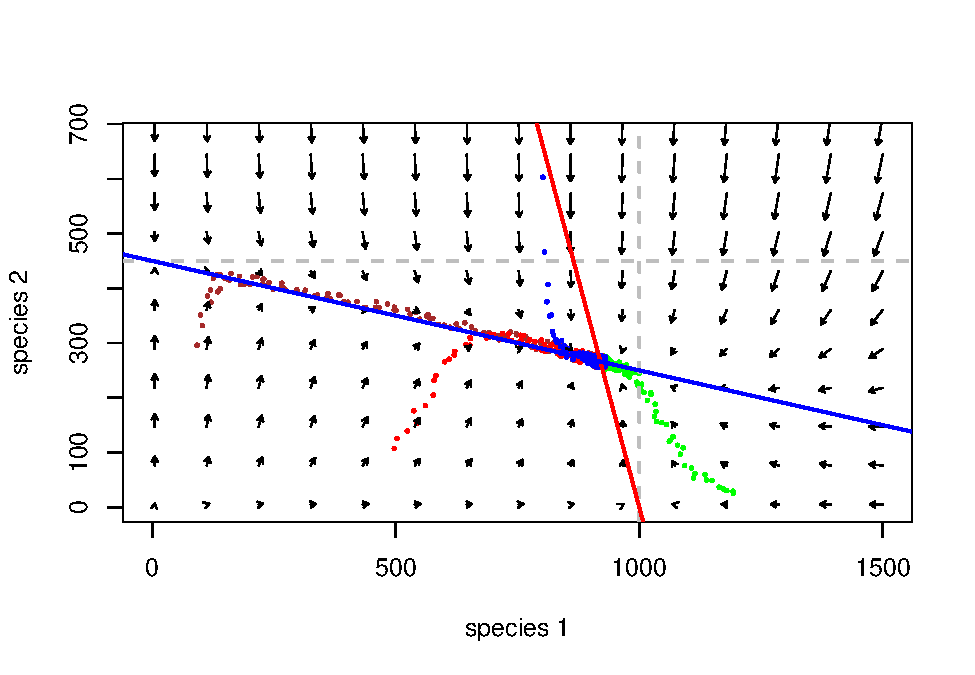
\includegraphics{LECTURE16_files/figure-latex/unnamed-chunk-15-1.pdf}

** P **: ¿En qué parte de esta figura se ``mueve'' el sistema más
rápido? (Analogía del campo magnético: atracción y repulsión más
fuertes)

Finalmente, considere este ejemplo:

\begin{Shaded}
\begin{Highlighting}[]
\DocumentationTok{\#\#\#\#\#\#\#\#}
\CommentTok{\# And finally...}
\DocumentationTok{\#\#\#\#\#\#\#\#}

\NormalTok{Rmax1 }\OtherTok{\textless{}{-}} \FloatTok{0.2}
\NormalTok{Alpha }\OtherTok{\textless{}{-}} \FloatTok{1.5}
\NormalTok{K1 }\OtherTok{\textless{}{-}} \DecValTok{1000}
\NormalTok{Rmax2 }\OtherTok{\textless{}{-}} \FloatTok{0.2}
\NormalTok{Beta }\OtherTok{\textless{}{-}} \DecValTok{2}
\NormalTok{K2 }\OtherTok{\textless{}{-}} \DecValTok{1500}

\NormalTok{parms}\OtherTok{=}\FunctionTok{c}\NormalTok{(Rmax1,Alpha,K1,Rmax2,Beta,K2)}

\CommentTok{\# toggle(100,100,parms)}

\NormalTok{xlim }\OtherTok{=} \FunctionTok{c}\NormalTok{(}\DecValTok{5}\NormalTok{,}\DecValTok{1500}\NormalTok{)}
\NormalTok{ylim }\OtherTok{=} \FunctionTok{c}\NormalTok{(}\DecValTok{5}\NormalTok{,}\DecValTok{1000}\NormalTok{)}
\NormalTok{new }\OtherTok{\textless{}{-}} \FunctionTok{phasearrows.calc}\NormalTok{(toggle,xlim,ylim,}\AttributeTok{resol=}\DecValTok{25}\NormalTok{,}\AttributeTok{parms=}\NormalTok{parms)}

\FunctionTok{plot}\NormalTok{(}\DecValTok{1}\NormalTok{,}\DecValTok{1}\NormalTok{,}\AttributeTok{pch=}\StringTok{""}\NormalTok{,}\AttributeTok{xlim=}\NormalTok{xlim,}\AttributeTok{ylim=}\NormalTok{ylim,}\AttributeTok{xlab=}\StringTok{"N1"}\NormalTok{,}\AttributeTok{ylab=}\StringTok{"N2"}\NormalTok{)}
\FunctionTok{phasearrows.draw}\NormalTok{(new)}
\FunctionTok{abline}\NormalTok{(K1}\SpecialCharTok{/}\NormalTok{Alpha,}\SpecialCharTok{{-}}\NormalTok{(K1}\SpecialCharTok{/}\NormalTok{Alpha)}\SpecialCharTok{/}\NormalTok{K1,}\AttributeTok{col=}\StringTok{"red"}\NormalTok{,}\AttributeTok{lwd=}\DecValTok{3}\NormalTok{)   }\CommentTok{\# species 1}
\FunctionTok{abline}\NormalTok{(K2,}\SpecialCharTok{{-}}\NormalTok{K2}\SpecialCharTok{/}\NormalTok{(K2}\SpecialCharTok{/}\NormalTok{Beta),}\AttributeTok{col=}\StringTok{"blue"}\NormalTok{,}\AttributeTok{lwd=}\DecValTok{3}\NormalTok{)   }\CommentTok{\# species 2}
\end{Highlighting}
\end{Shaded}

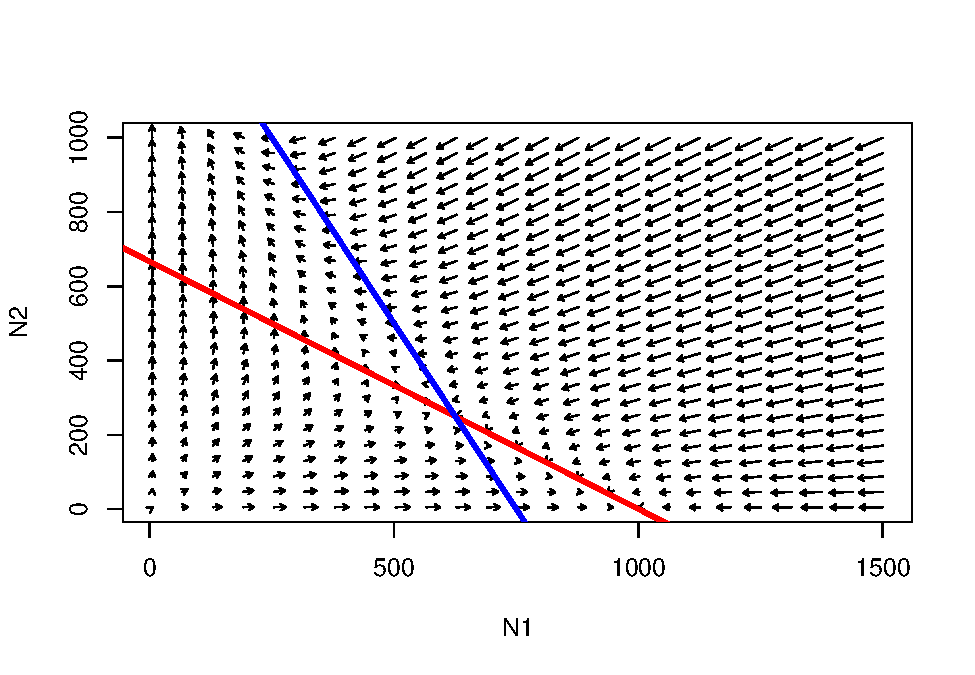
\includegraphics{LECTURE16_files/figure-latex/unnamed-chunk-16-1.pdf}

\textbf{P }: ¿es el punto donde las dos isoclinas cruzan un * equilibrio
*?

\textbf{P }: ¿es el punto donde las dos isoclinas cruzan un * equilibrio
estable *?

\textbf{P }: ¿qué pasaría si la especie 1 estuviera en K y la especie 2
intentara invadir? ¿Y viceversa?

\textbf{P }: ¿qué pasaría si ambas especies intentaran invadir un
hábitat vacío al mismo tiempo?

\hypertarget{phase-space-in-insightmaker}{%
\subsubsection{Phase space in
InsightMaker}\label{phase-space-in-insightmaker}}

You can visualize populations moving through the phase plane in
InsightMaker! To do this, just click on ``Add Display'' in the graphics
window (which comes up automatically when you hit ``Simulate'') and
create a ``Scatter Plot''. For the ``Data'' field, select the two stocks
(species abundances).

If you don't already have a working L-V competition model you can load
up the basic L-V competition model
\href{https://insightmaker.com/insight/77730/Competition-1\#}{here}

\textbf{Step 1}: Set the key parameters (alpha, beta, K1, K2) to
arbitrary values

\textbf{Step 2}: Draw out the phase plane with isoclines for both
competing species.. Also draw out the expected direction of growth in
each quadrant/region of the phase plane.

\textbf{Step 3}: Pick an arbitrary starting value. What do you think the
trajectory is going to look like?

\textbf{Step 4}: Run this model in InsightMaker. Does the system behave
as expected?

\textbf{Step 5}: Evaluate the following statement (from the Gotelli
Book):

\begin{quote}
``the more similar species are in their use of shared resources, the
more precarious their coexistence''
\end{quote}

\textbf{Q}: Does \(r_{max}\) have any role to play in determining system
stability for the lotka-volterra competition model?

\href{LECTURE17.html}{--go to next lecture--}

\end{document}
